\section{Transport Layer}


\subsection{TCP}

\subsubsection{Header}

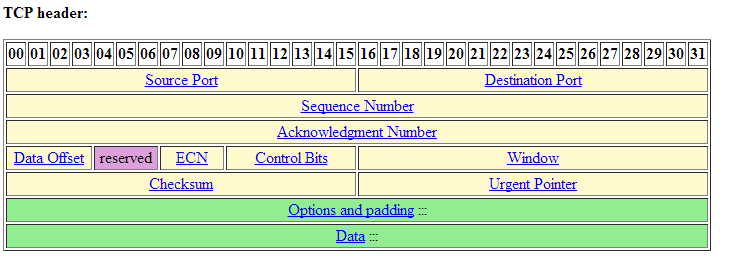
\includegraphics[width=\textwidth]{media/TCPHeader.png}

Aufgepasst: Die Checksumme berücksichtigt auch den IP-Header und verletzt somit
das Schichten Modell.

\begin{align*}
	Maximum Segment Size (MSS) = MTU - IPHeader - TCP Header & = \textrm{1460 Byte}\\
	MTU &= \textrm{1500 Byte}\\
	IPHeader &= \textrm{20 Byte}\\
	TCPHeader &= \textrm{min 20 Byte}
\end{align*}

\subsubsection{3 Way Handshake}

\begin{minipage}{.4\linewidth}
	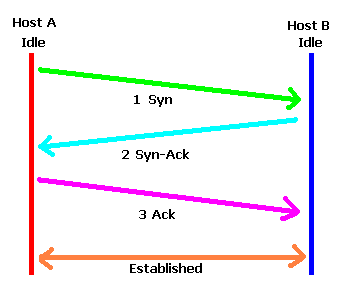
\includegraphics[width=\textwidth]{media/3way.png}
\end{minipage}
\begin{minipage}{.6\linewidth}
	\begin{enumerate}
		\item Host A sends a TCP \textbf{SYN}chronize packet to Host B.
		\\ Host B receives A's \textbf{SYN}.
		\item Host B sends a \textbf{SYN}chronize-\textbf{ACK}nowledgement.
		\\ Host A receives B's \textbf{SYN-ACK}.
		\item Host A sends \textbf{ACK}nowledge.
		\\ Host B receives \textbf{ACK}.
	\end{enumerate}
\end{minipage}


\subsubsection{Connection Closing}

\begin{minipage}[t]{.4\linewidth}
	\vspace{0pt}
	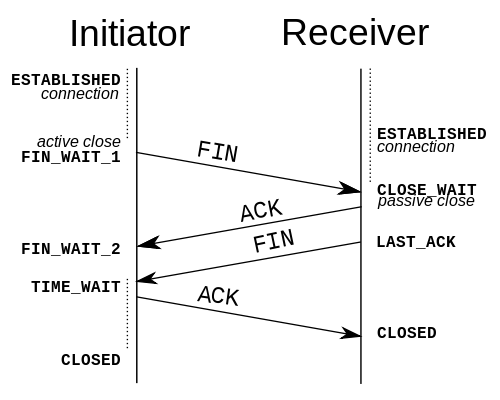
\includegraphics[width=\textwidth]{media/tcp_connection_closing.png}
\end{minipage}
\hspace{5mm}
\begin{minipage}[t]{.5\linewidth}
	\vspace{0pt}
	Für die Terminierung einer Verbindung wird ein 4 Way Handshake (FIN, ACK, FIN,
	ACK) verwendet.

	Alternativ ist es auch möglich, die Verbindung mit einem 3 Way Handshake (FIN,
	FIN-ACK, ACK) zu schliessen.
\end{minipage}


\subsubsection{Analyse TCP Stream}

\begin{minipage}[t]{0.5\linewidth}
	\textbf{Cumulative ACK}

	\vspace{5mm}

	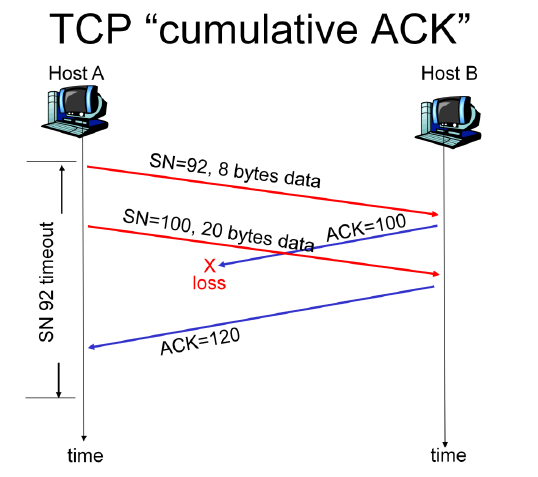
\includegraphics[width=0.9\textwidth]{media/cumulativeACK.png}
\end{minipage}
\begin{minipage}[t]{0.5\linewidth}
	\textbf{Delayed ACK}

	\vspace{5mm}

	Im Prinzip wie Cumulative ACK. Die ACK Verluste sind aber absichtlich, d.h der
	Empfänger sendet nicht für jedes Paket ein ACK, sondern wartet auf eine der 2
	Bedingugen:

	\begin{enumerate}
		\item TCPDelAckTicks: Ist nach Ablauf dieses Timers kein Paket mehr
			angekommen, sendet er ein kumulatives ACK.
		\item TCPAckFrequency: Wurde für die festgelegte Anzahl Pakete kein ACK
			versendet, sendet er ein kumulatives ACK.
	\end{enumerate}
\end{minipage}

\subsubsection{TCP Flow Control}

\textbf{Window Size}

Mit dem Receive Window (RWin) gibt der Empfänger dem Sender an, wie viele Bytes
der Sender noch schicken darf, ohne ein ACK erhalten zu haben. Receive Window
ist die Receive Buffer Grösse des Empfängers.

Das Ziel ist es die Pipe zwischen Sender und Empfänger immer optimal zu füllen,
sodass der Sender nicht auf ACKs warten muss. Die Window Size sollte grösse
sein als RTT * Bandbreite.

Schickt der Sender das erste Paket ab, dauert es eine RTT bis er ein ACK
bekommt. Während dieser Zeit sollte der Sender aber fortlaufend weitere Pakete
in die Pipe legen dürfen. Oder anders gesagt, die Anzahl Pakete die der Sender
während einer RTT in die Pipe legen kann ist das BDP (Bandwidth Delay Product).
Die Window Size sollte optimalerweise mindestens so gross sein wie das BDP, da
sonst auf ACKs gewartet werden muss.

$BDP=RTT \cdot Bandwidth$

Beispiel Kommunikation nach Thailand:
\[
	R_{win} = \SI{50000}{\kibi\bit\per\second} \cdot \SI{.3}{\second} = \SI{150000}{\kibi\bit} = \SI{1875}{\kibi\byte}
\]

\textbf{Maximale Distanzen}

Nachfolgend ein Beispiel für die Maximale Distanz (Füllung der Pipe) bei
gegebener Window Size von 64 KiB und Geschwindigkeit von 1.5 MiBit/s.
\[
	RTT = \frac{R_{win}}{R_{max}}\\
\]
\[
	\frac{\SI{64}{\kibi\byte} \cdot \SI{8}{\bit\per\byte} \cdot
	\SI{1024}{\bit\per\kibi\byte}}{\SI{1.5}{\mebi\bit\per\second}} = \SI{.35}{s}
\]
\[
	Distance = v \cdot t =\left(\frac{2}{3} \cdot \SI{300000}{\kilo\meter\per\second}\right)\cdot \SI{.35}{s} = \SI{70000}{\kilo\meter}
\]

\textbf{Duplicate Acknowledgement}

Der Empfänger sendet ein Dup ACK (Acknowledgment, dass er bereits gesendet hat),
d.h ein Paket vom Sender muss verloren gegangen sein. Nach 3 Dup ACKs (4
Identischen ACKs ohne weitere Pakete dazwischen, sendet der Sender das
verlorengegangene Paket nochmals.

\textbf{Fast Retransmit}

Sobald ein Paket Out-of-Order empfangen wird, wird sofort ein Dup ACK gesendet.
Die Pakete die in der Zwischenzeit beim Empfänger ankommen werden jedoch
behalten und nach einem allfälligen Retransmit kumulativ bestätigt.

Ein Dup ACK heisst, dass ein Paket Out-Of-Order ist, wobei 3 Pakete ein ziemlich
sicheres Indiz für ein Paketverlust ist.

\textbf{Selective ACK}

Die SACK Option muss beim Verbindungsaufbau im SYN aktiviert werden. 

Ein ACK mit SACK beinhaltet Block mit Daten, die bereits erfolgreich empfangen
wurden. D.h die Daten unterhalb (ACK - beginn des Blocks) und oberhalb des
Blocks müssen nochmals versandt werden. Die Blockstart bzw. end Oktett angaben
werden mittels 32Bit Werten dargestellt. Ein Bock ist also 8 Bytes gross.

Die Maximalgrösse des TCP Headers ist 40 Bytes, demnach sind maximal 4 Blöcke
(32Bytes) + Option Type / LEN (2Bytes) pro Paket möglich. Jedoch wird in diesem
Zusammenhang auch noch die RTTM Option verwendet welche 10 + 2 Bytes benötigt
verwendet. Somit bleibt nur noch für 3 Blöcke Platz.

\textbf{Congestion Window (CWND) / Slow Start}

Das Congestion Window ist die Flusskontrolle auf Senderseite im Gegensatz zur
Window Size welche die Flusskontrolle auf Empfängerseite darstellt. Die CWND
Size wird jedoch nicht kommuniziert, sie stellt nur eine lokale Kontrollgrösse
dar. Die CWND legt die Anzahl Segmente fest, welche ohne ACKs gesendet werden
können. Die MSS (Maximum Segment Size) wird vom Empfänger mittgeteilt. Zu Beginn
ist dieser Wert 1 (Slow Start) und wird nach jedem ACK erhöht. Schlussendlich
gilt der kleinere Wert $min(cwnd,WindowSize)$ als MaxWin Size und bestimmt
wieviele Segmente ohne ACKs höchstens gesendet werden dürfen.

\subsubsection{TCPTrace}

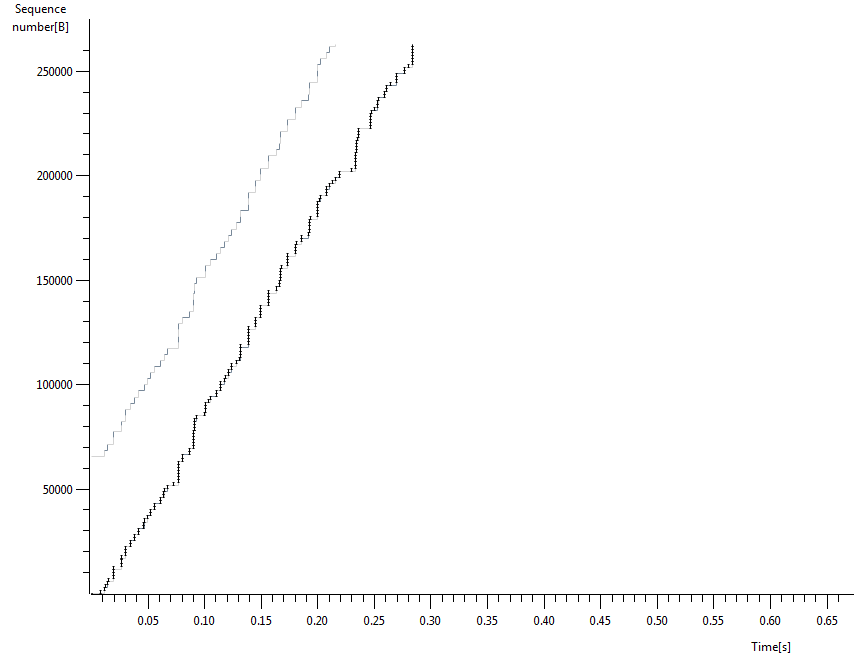
\includegraphics[scale=0.45]{media/tcptraceUpload.png}

Anhand der schnell ansteigenden Sequenznummern ist zu erkennen, dass es sich um
einen Upload handelt.

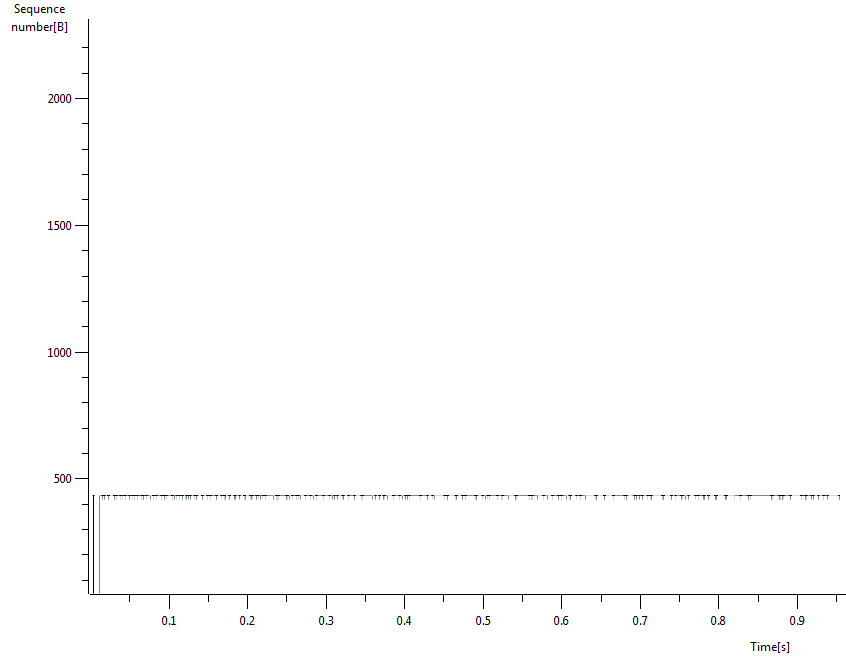
\includegraphics[scale=0.45]{media/tcptraceDownload.png}

Anhand der nur langsam erhöhenden Sequenznummer ist zu erkennen, dass nur sehr
wenige Daten versendet werden und es sich somit um einen Download handelt.

\textbf{Wo wurde der Trace aufgezeichnet}

Anhand der verstrichenen Zeit zwischen einer Datenpaket-Sequenz und dem
dazugehörigen ACK ist zu erkennen, ob der Wireshark Trace auf Client oder
Serverseite aufgezeichnet wurde. Wird ein Upload (Server->Client) auf der
Clientseite aufgezeichnet, sind die ACKs kaum zu erkennen, da sie gleich nach
dem Empfangen (<1ms) abgeschickt werden.

\subsubsection{Vorteile gegenüber UDP}

\begin{enumerate}
	\item Verbindunsorientierung (SYN/ACK)
	\item Zuverlässiger Transport (Sequenznummern und Acknowledgements)
	\item Stauvermeidung (Congestion Window)
	\item Flusskontrolle (Receive Window Size)
\end{enumerate}


\subsection{UDP}

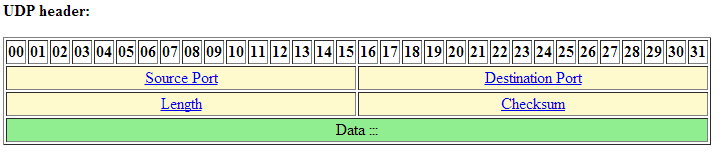
\includegraphics[width=\textwidth]{media/UDPHeader.png}

Aufgepasst: Die Checksumme berücksichtigt auch den IP-Header und verletzt somit
das Schichten Modell.

Das Längenfeld beinhaltet auch den UDP Header, ist also immer mindestens 8.

\begin{align*}
Maximum Segment Size (MSS) = MTU - IPHeader - UDP Header &= 1472\\
MTU &= \SI{1500}{\byte}\\
IPHeader &= \SI{20}{\byte}\\
UDPHeader &= \SI{8}{\byte}
\end{align*}

\subsubsection{Analyse UDP Stream}

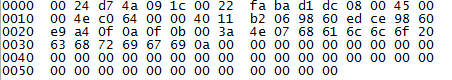
\includegraphics[scale=1.0]{media/UDPStream.png}

\textbf{MAC Header}

\begin{tabular}[h]{|l|l|}
	\hline
	DST Address: & 00:24:D7:4A:09:1C \\
	\hline
	SRC Address: & 00:22:FA:BA:D1:DC \\
	\hline
	Ethertype: & 0x8000 (IP) \\
	\hline
\end{tabular}

\textbf{IP Header}

\begin{tabular}[h]{|l|l|}
	\hline
	Version \& IHL: & 0x45 (Version 4, IHL 5) \\
	\hline
	TOS: & 0x00 \\
	\hline
	Total Length: & 0x004e (78 Bytes) \\
	\hline
	Identification: & 0xC064 (49252) \\
	\hline
	Flags \& Offset: & 0x0000 \\
	\hline
	TTL: & 0x40 (128) \\
	\hline
	Protocol: & 0x11 (17/UDP) \\
	\hline
	Checksum: & 0xB206 \\
	\hline
	Src Address: & 0x98.0x60.0xED.0xCE (152.96.237.206) \\
	\hline
	Dst Address: & 0x98.0x60.0xE9.0xA4 (152.96.233.164) \\
	\hline
	Option \& Padding: & - \\
	\hline
\end{tabular}

\textbf{UDP Header}

\begin{tabular}[h]{|l|l|}
	\hline
	Source Port: & 0x0F0A (3850) \\
	\hline
	Destination Port: & 0x0F0B (3851) \\
	\hline
	Length: 0x003A & (58 Bytes) \\
	\hline
	Checksum: & 0x4E07 \\
	\hline
	Data: & hallo chrigi00000000.... (50 Bytes) \\
	\hline
\end{tabular}
